\documentclass[a4paper,12pt]{article}

\usepackage[utf8]{inputenc}
\usepackage[MeX]{polski}
\usepackage{fullpage}
\usepackage{graphicx}

\title{\LARGE{[SDPB] Wyznaczanie trasy} \\ \vspace{2mm} \large{Dokumentacja końcowa projektu}}
\author{Michał Aniserowicz, Jakub Turek}
\date{}

\begin{document}
	\maketitle

	\section*{Temat projektu}

	Napisać aplikację wyznaczającą i~porównującą trasę przejazdu na terenie Warszawy środkami komunikacji miejskiej i~samochodem z~opcją ustawienia godziny wyjścia z~domu żeby zdążyć na czas. Aplikacja może być aplikacją mobilną lub przeznaczoną na komputer klasy PC.

	\section*{Założenia}

	Temat został uszczegółowiony poniższymi założeniami:

	\begin{itemize}
		\item Aplikacja zaprojektowana w~architekturze klient-serwer.
		\item Serwer posiada dwie odpowiedzialności:
		\begin{itemize}
			\item Przechowuje dane.
			\item Dostarcza logikę związaną z~przeliczaniem tras.
		\end{itemize}
		\item Klient jest aplikacją dostępową umożliwiającą wprowadzenie następujących danych:
		\begin{itemize}
			\item Lokalizacja początkowa i~docelowa (punkty na mapie).
			\item Docelowy czas przyjazdu.
			\item Przejazd komunikacją miejską lub samochodem.
		\end{itemize}
		\item Klient na wyjściu prezentuje najszybszą trasę dla podanych danych wejściowych oraz godzinę wyjścia/wyjazdu, która pozwala zdążyć na czas.
		\item Dane nie są dostarczane z~systemów zewnętrznych (np. \emph{Google Maps}, \emph{Jak dojadę}), ale składowane w~bazie danych opracowanej w~ramach projektu.
		\item Uproszczenie algorytmu wyznaczania trasy:
		\begin{itemize}
			\item Założenie, że czas przejazdu tego samego odcinka drogi komunikacją miejską i~samochodem jest identyczny.
			\item Brak uwzględnienia informacji o~godzinach przyjazdu środków komunikacji miejskiej na przystanki. Zakłada się, że czas wymagany na przesiadkę jest stały i~jest parametrem algorytmu.
			\item Wyznaczana jest zawsze pojedyncza najszybsza trasa dla wybranego środka komunikacji.
			\item Jako punkt początkowy i~końcowy wybierane są te lokalizacje spośród danych znajdujących się w~bazie, które są najbliższe lokalizacjom wskazanym przez użytkownika.
			\item W~przypadku wskazania komunikacji miejskiej jako środka transportu punktem początkowym i~końcowym podróży są zawsze przystanki najbliższe wskazanym lokalizacjom. Nie jest uwzględniana możliwość dojścia do przystanku.
		\end{itemize}
	\end{itemize}

	\section*{Architektura aplikacji}

	Aplikacja została zaprojektowana w~architekturze klient-serwer. Szczegółowy schemat architektury przedstawia rysunek~\ref{fig:architecture}. 

	\begin{figure}[ht!]
		\centering
		\scalebox{0.7}[1.0]{
			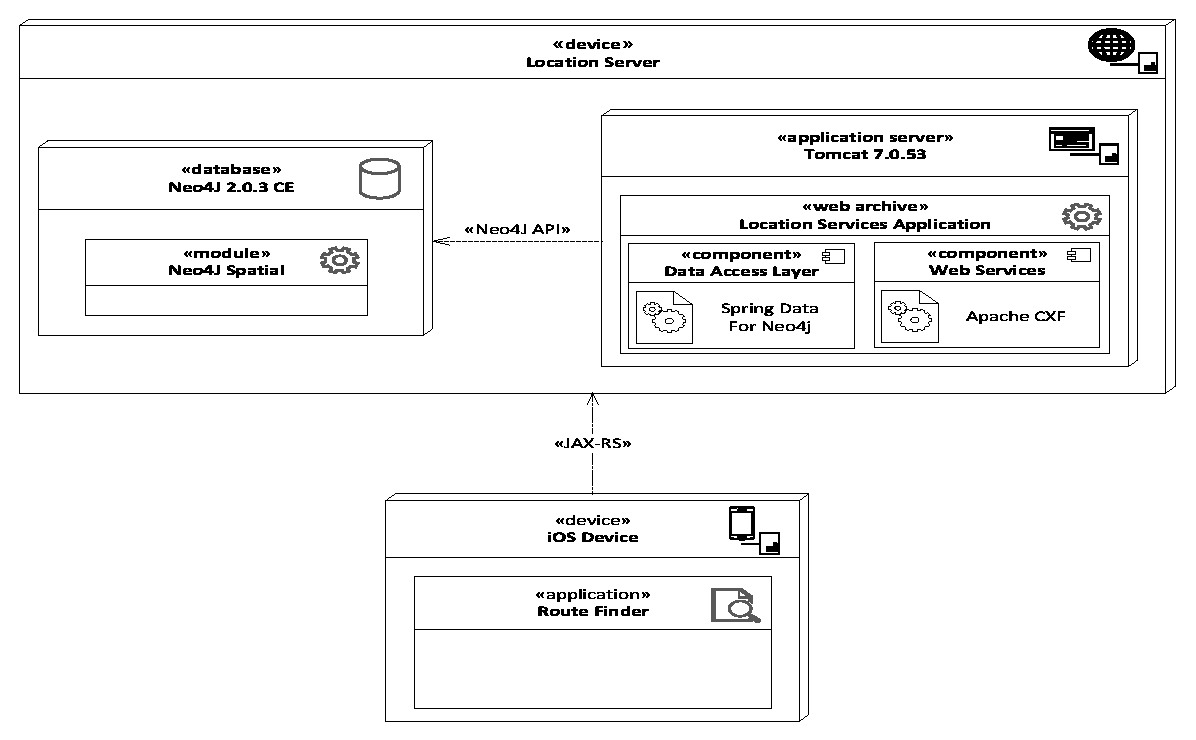
\includegraphics{graphics/architecture.eps}
		}

		\caption{Schemat architektury aplikacji.}
		\label{fig:architecture}
	\end{figure}

\end{document}
